\begin{frame}
	\frametitle{
		Método de continuación homotópica para solucionar sistemas no
		lineales
	}

	El problema de solucionar numéricamente un sistema de $n$
	ecuaciones no lineales en $n$ variables $F\left(x\right)=0$
	donde
	\begin{math}
		F\colon\mathbb{R}^{n}\to\mathbb{R}^{n}
	\end{math}
	aparece ampliamente en cálculos científicos.
	Suponga que $F$ es suave, es decir, tiene tantas derivadas
	parciales continuas como se requiera.
	Un algoritmo conocido para este problema son las
	\alert{iteraciones de Newton}:
	\begin{equation*}
		x^{\left(n+1\right)}=
		x^{\left(n\right)}-
		{\left(DF\left(x^{\left(n\right)}\right)\right)}^{-1}
		F\left(x^{\left(n\right)}\right),\quad
		n=0,1,2,\dotsc,\quad
		x^{\left(0\right)}\in\mathbb{R}^{n}
	\end{equation*}
	donde
	\begin{math}
		DF\left(x^{\left(n\right)}\right)
	\end{math}
	es la \alert{matriz jacobiana} de $F$ en $x^{\left(n\right)}$.
	Este algoritmo es \alert{local} en el sentido de que se requiere
	una muy buena estimación de la solución correcta para la
	convergencia del algoritmo.
	Desafortunadamente, tal conocimiento sobre los de $F$ no suele
	estar disponible a priori.
	Como posible remedio, se define

	\begin{definition}[homotopía]
		Una \alert{homotopía} (suave) entre dos funciones continuas
		(suaves)
		\begin{math}
			G\colon
			\mathbb{R}^{n}\to
			\mathbb{R}^{n}
		\end{math}
		(sistema origen) y
		\begin{math}
			F\colon
			\mathbb{R}^{n}\to
			\mathbb{R}^{n}
		\end{math}
		(sistema destino) es definida como una función continua (suave)
		\begin{math}
			H\colon
			\left[0,1\right]\times\mathbb{R}^{n}\to
			\mathbb{R}^{n}
		\end{math}
		sii
		\begin{equation*}
			\forall x\in\mathbb{R}^{n}:
			H\left(0,x\right)=
			G\left(x\right),\quad
			H\left(1,x\right)=
			F\left(x\right)
		\end{equation*}
		y los ceros de $G\left(x\right)=0$ se obtienen fácilmente.
		Sea $x_{0}$ un cero de $G\left(x\right)=0$.
		Entonces, si
	\end{definition}

	\begin{columns}
		\begin{column}{0.48\textwidth}
			\begin{itemize}
				\item

				      \begin{math}
					      t=0:
					      H\left(0,x\right)=
					      0
				      \end{math}
				      tiene una única solución $x=x_{0}$.

				\item

				      \begin{math}
					      t=1:
					      H\left(1,x\right)=
					      0
				      \end{math}
				      concuerda con
				      $F\left(x\right)=0$.
			\end{itemize}
		\end{column}
		\begin{column}{0.48\textwidth}
			\begin{itemize}
				\item

				      $t\in\mathbb{R}: x\left(t\right)$ es solución de
				      $H\left(t,x\left(t\right)\right)=0$, entonces bajo
				      ciertas condiciones generará una curva suave.
			\end{itemize}
		\end{column}
	\end{columns}

	\

	Si uno puede trazar con éxito esta curva suave $x\left(t\right)$
	desde $t=0$ donde $x\left(0\right)=x_{0}$ continuamente, entonces
	cuando $t=1$, se obtiene una solución $x\left(1\right)=x$
	de $F\left(x\right)=0$.
\end{frame}

\begin{frame}
	\begin{alertblock}{Interpretación geométrica de la homotopía}
		Se puede considerar como una deformación entre dos sistemas
		$G\left(x\right)$ y $F\left(x\right)$ dentro una familia de
		sistemas.
		La curva solución definida por
		\begin{math}
			H\left(t,x\right)=0
		\end{math}
		a partir del punto
		\begin{math}
			\left(0,x_{0}\right)
		\end{math}
		conducirá a soluciones al sistema de interés
		\begin{math}
			F\left(x\right)=
			0
		\end{math}
		cuando esta curva suave cruce el plano
		\begin{math}
			\left[0,1\right]\times\mathbb{R}^{n}
		\end{math}
		definida por $t=1$.
	\end{alertblock}
	\begin{figure}[ht!]
		\centering
		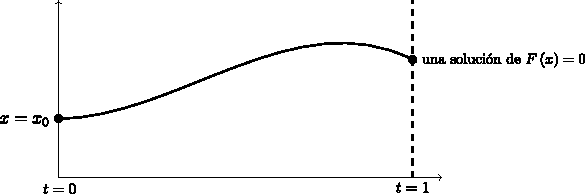
\includegraphics[width=0.65\paperwidth]{homotopy}
		\caption{
			Una curva suave definida por $H\left(t,x\right)=0$ alcanzando
			una solución $x^{\ast}$ del sistema objetivo.
		}
	\end{figure}

	\begin{definition}[Valor regular]
		Sea $F\colon\mathbb{R}^{n}\to\mathbb{R}^{p}$ suave.
		Un punto $y\in\mathbb{R}^{p}$ es \alert{valor regular} de $F$ sii
		% \coloneqq\left\{x\in\mathbb{R}^{n}\mid F\left(x\right)=y\right\}
		\begin{math}
			\forall x\in F^{-1}\left(\left\{y\right\}\right):
			\operatorname{Imag}\left(DF\left(x\right)\right)=
			\mathbb{R}^{p}
		\end{math}.
		% donde $DF\left(x\right)\in\mathbb{R}^{n\times p}$ es la matriz
		% jacobiana de $F$, que consiste de todas las derivadas parciales
		% de $F\left(x\right)$ con respecto a
		% $x=\left(x_{1},\dotsc,x_{n}\right)$.
	\end{definition}

	$0\in\mathbb{R}^{n}$ es un valor regular de $H$ siempre que
	la matriz jacobiana $DH\in\mathbb{R}^{n\times n+1}$ de $H$ con
	respecto a $\left(t,x\right)$ es de rango $n$ (rango fila completo)
	para cualquier
	\begin{math}
		\left(x,t\right)\in
		H^{-1}\left(\left\{0\right\}\right)\subset
		\left[0,1\right]\times\mathbb{R}^{n}
	\end{math}.
	Esta condición permite la continuación de una solución de un solo
	sistema en la deformación en una curva solución.
\end{frame}